% Code Source: https://tex.stackexchange.com/questions/644238/drawing-the-phase-portrait-of-two-differential-equations
\pgfplotsset{ % Define a common style, so we don't repeat ourselves
	DGLRf/.style={
		width=0.6\textwidth, % Overall width of the plot
		axis equal image, % Unit vectors for both axes have the same length
		view={0}{90}, % We need to use "3D" plots, but we set the view so we look at them from straight up
		xmin=0, xmax=1.1, % Axis limits
		ymin=0, ymax=1.1,
		domain=0:1, y domain=0:1, % Domain over which to evaluate the functions
		xtick={0,0.5,1}, ytick={0,0.5,1}, % Tick marks
		samples=11, % How many arrows?
		cycle list={    % Plot styles
			gray,
			quiver={
				u={1}, v={f(x)}, % End points of the arrows
				scale arrows=0.075,
				every arrow/.append style={
					-latex % Arrow tip
				},
			}\\
			red, samples=31, smooth, thick, no markers, domain=0:1.1\\ % The plot style for the function
		}
	}
}
\begin{tikzpicture}[
	declare function={f(\x) = 2*\x;} % Define which function we're using
	]
	\begin{axis}[
		DGLRf, title={$\dfrac{\mathrm{d}y}{\mathrm{d}x}=2x$}
		]
		\addplot3 (x,y,0);
		\addplot {x^2+0.15} node[near start] {$\bullet$} node[near start, right] {$(x_1,y_1)$}; % You need to find the antiderivative yourself, unfortunately. Good exercise!
		\addplot {0};
		\addplot {x^2+0.3};
		\addplot {0};
		\addplot {x^2+0.45}  node[near start] {$\bullet$} node[near start, left] {$(x_0,y_0)$};
	\end{axis}
\end{tikzpicture}